\chapter{Implementation details}

How was mentioned above for working with images it was decided to use opencv library. It is more flexible to use and its core is based on C++. Nowadays C++ is one of the most efficient language. The algorithms in opencv are implemented with a very good asymptotic of time. Like in any programming languages in c++ we need to start with main part. In opencv to read the video in is enough to use the VideoCapture class where are implemented everything for streaming from the video. It is enough to give for it the filename and it will work with a ready video which was preliminarily recorded. At the line where in the parameters of cap is given 0 is used to say for a CPU that it is going to use web camera of the used system. The code is described in Figure \ref{fig:main_of_code}

\begin{figure}[h!]
    \centering
    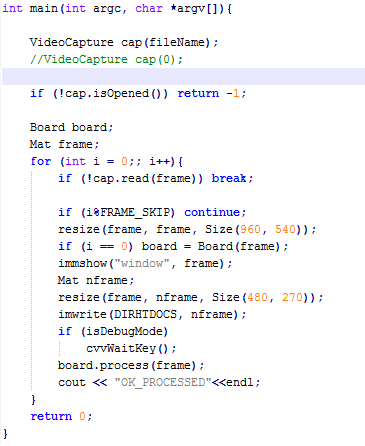
\includegraphics[]{Figures/main_of_code}
    \caption{main function}
    \label{fig:main_of_code}
\end{figure}

Further in the object created from the class VideoCapture is checked for error. Exactly, can it open the video or not. If no it will close the application. Then in a cycle it is written to read each frame and skip for \verb|FRAME_SKIP| size. The modulo was used to observe only those images which are dividable for a \verb|FRAME_SKIP|. Then it will take each \verb|FRAME_SKIP|*i’s frame for further processing. The resize of the window was used to make for comfortable for debugging and have a fixed size for any video.
	
	
There are also used two structures. They are Board and Mat. The Board structure is described in a Figure \ref{fig:board_structutre}

\begin{figure}[h]
    \centering
    \includegraphics[]{Figures/board_structutre}
    \caption{Board struct}
    \label{fig:board_structutre}
\end{figure}

For completely detecting the board there are used several states. 

The \verb|IND_BOARD_INITIAL_STATE| = 0 is waiting for hand cover state. 

The \verb|FIND_BOARD_WAITING_FOR_CHANGES| = 1 is for the state where takes the board matrix and waits for the next hand cover. 

\verb|FIND_BOARD_FOUND_BOARD| = 2 is used when all the board points are found.

\verb|MAX_DEVIATION| = 100 more value is give more motion is allowed. The line

\verb|MOTION_CHANGES| = 10 is the percentage of big motion.

For detecting the hand cover there was used a solution like this: 

Each \verb|FRAME_SKIP| frame there is calculated the changes by using the Collin’s algorithm. After the threshold we have the changes. Then it is compared if the percentage of the changes are more than \verb|HAND_COVER_PERCENT| is will recognize it as hand cover and move the state to the next state. When the constructor is called the state is initialized to \verb|FIND_BOARD_INITIAL_STATE|;

In the Figure \ref{fig:process_method} is described the method process which is called first in main body of the application. 

\begin{figure}[h]
    \centering
    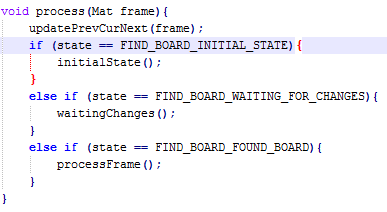
\includegraphics[]{Figures/process_method}
    \caption{process method}
    \label{fig:process_method}
\end{figure}


In this method checks and calls methods to its corresponding states. In the theoretical part was described the depth first search algorithm. This algorithm is used to separate the point into components. The dfs algorithm is recursive function which call itself each time. The algorithm is described in Figure \ref{fig:dfs_algo}

\begin{figure}[h]
    \centering
    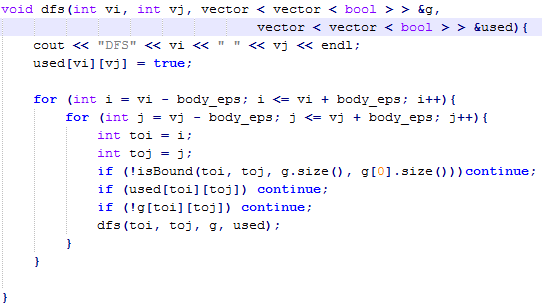
\includegraphics[width=\textwidth]{Figures/dfs_algo}
    \caption{Depth-first-search algorithm}
    \label{fig:dfs_algo}
\end{figure}

After the finding all the components by using the dfs algorithm they should be checked for rectangle shape. In Figure \ref{fig:check_rect} shown the implementation of check.

\begin{figure}[h]
    \centering
    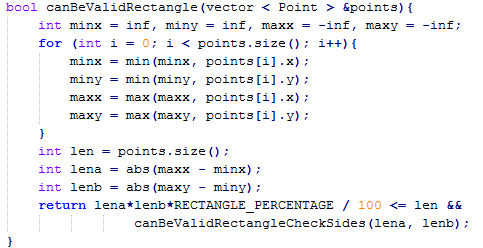
\includegraphics[]{Figures/check_rect}
    \caption{Function to check the points for rectangle shape}
    \label{fig:check_rect}
\end{figure}


As an input this function takes collections of points. Then bounding box is used to determine the borders of the rectangle. This bounding box is send to the another function to check if this bounding box can be a valid rectangle. In function canBeValidRectangleCheckSides was implemented the check for perimeters and diagonals. After the detecting all the edges of the board it will track the changes on the board and send all the changes to the server. First, its needed to detect if the board’s edges are destroyed or not. If not then we can move further. To detect is a human’s body inside of the board or outside it was used Canny’s algorithm to detect contours. Then the application checks whether one of the contours crosses the edges of the board. The edges of the board are drawn in a virtual memory. The edges of the whiteboard will the connected segments between the vertexes of the board. The vertexes are the four rectangles which were drawn at the beginning of the application when we say how large the rectangle is. It is obvious that Canny’s algorithm uses double threshold to give the result. As a minimum threshold was chosen the value 5. And as a maximum value was chosen 255. 
Figure \ref{fig:canny_edge_detection} 

\begin{figure}[h]
    \centering
    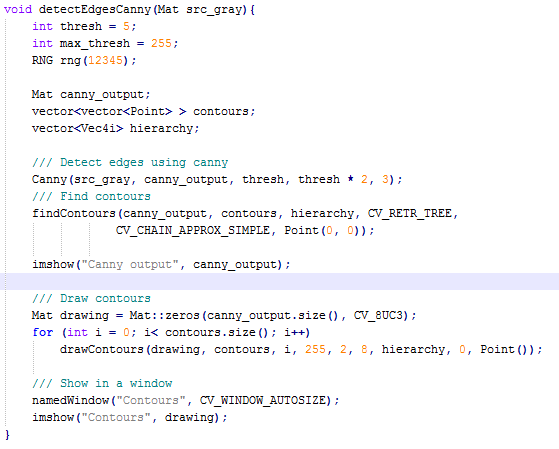
\includegraphics[]{Figures/canny_edge_detection}
    \caption{Edge detection algorithm using Canny}
    \label{fig:canny_edge_detection}
\end{figure}

It means it will make disappear if the value is less than 5 and point as strong if the value is more than max\_thresh (255). And as a weak if the value is between two values. First we detect edges and then find contours. There is a ready implemented Canny’s algorithm which gives the results as a picture. It is enough to give for a parameters minimum and maximum thresholds. Then after the getting the image from edge detection algorithm the application sends it to the findContours method. After the finding all the edges it is easy to check if the one of the edges which comes from outside crosses the edge of the board. In Figure \ref{fig:greedy_algorithm} is an implementation of greedy approach of compressing data.


\begin{figure}[h]
    \centering
    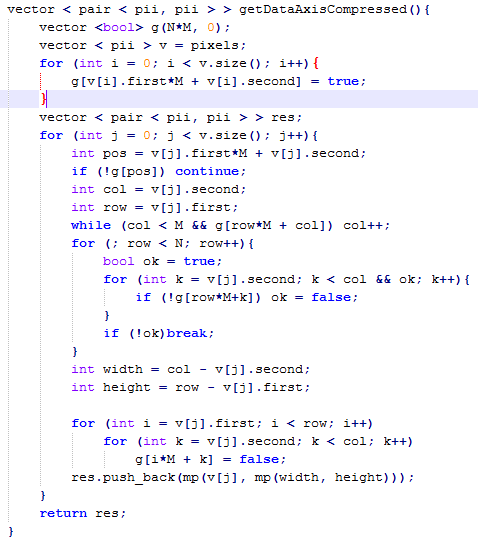
\includegraphics[]{Figures/greedy_algorithm}
    \caption{Greedy algorithm}
    \label{fig:greedy_algorithm}
\end{figure}


We have an image which contains from white and black pixels. We only interested in black pixels. Because we send only black pixels to the server. So we store the coordinates of black pixels in the array. So we have a sorted array of pixels (sorted first by rows then by columns). From this collection we take the top-left pixel that is not covered by any other rectangle. We take exactly top-left pixel because it is obvious that it will be one corner of our rectangle, especially the top-left corner of our current looking rectangle. Then we act greedily. We find as biggest rectangle as possible with a size (1, C) where all the pixels are black pixels. Here we find the width of our current covering rectangle. Now we want to find the Height of that rectangle. Now we find maximal R, such that from our starting coordinate. Lets define them as rowCord, colCord, and with a HEIGHT equal to R and WIDTH equal to C we have only black pixels inside this rectangle. So, actually we find one rectangle. Then we just erase the pixels inside this rectangle, and never consider them again. So, each time we only consider active black pixels which are not covered by any other rectangles. Then, we only once make them inactive. So total time complexity would be O(Number of Points) or O(length of black pixel array)



